\chapter{Problemdomäne Pressenplanung}
\label{chapter:problem}
In diesem Kapitel wird das Problem der Pressenplanung zunächst erläutert,
bevor die prädikatenlogische Modellierung des Problems in zwei Modellen erfolgt.
Abschließend werden die Modelle um Optimierungsziele erweitert.

\section{Anforderungen}
Im Pressenplanungsproblem sind drei Entitäten und deren Eigenschaften von elementarer Bedeutung: Pressen, Balken und Bauteile.
Diese haben jeweils die Eigenschaften Höhe, Breite und Länge.
Zusätzlich gibt es Holzlamellen, welche durch Zersägen eines sogenannten \textit{Endlosbretts} entstehen.
Dieses kann von einer Maschine \textit{scheinbar} endlos ausgegeben werden.
Höhe und Breite der Lamelle sind fest.
Lamellen werden vertikal zu Bauteilen verleimt, sodass Bauteile immer die Form eines Quaders haben.
Diese Verleimung ist der eigentliche Grund für die Notwendigkeit des Pressens. \sem{Ruhig den Prozess, wie aus einem Brett ein Bauteil ensteht beschreiben. Versuche am Anfang den Prozess von der Modellierung zu trennen.}
Folgend eine Abbildung verleimter Lamellen:

\begin{figure}[h]
    \centering
    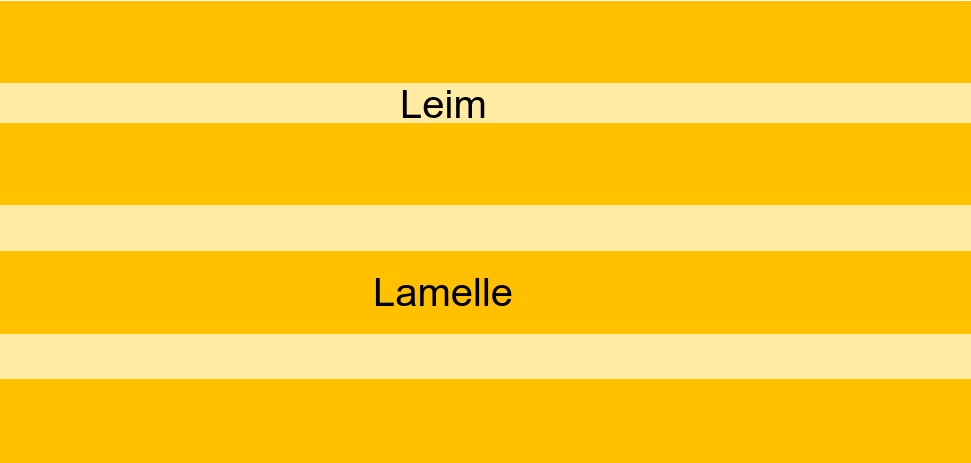
\includegraphics[width=0.70\textwidth, center]{Images/LammelleLeim}\\
    \caption{Vertikale Verleimung von Lamellen \sem{Vollständige Bildbeschreibung}}
    \label{figure:lamelleleim}
\end{figure}

Bauteile wiederum formen Balken - ebenfalls Quader.
Bauteile erhält man durch vertikales Zersägen eines Balkens.
Folgend eine Abbildung eines Balkens aus drei Bauteilen mit Rest:

\begin{figure}[h]
    \centering
    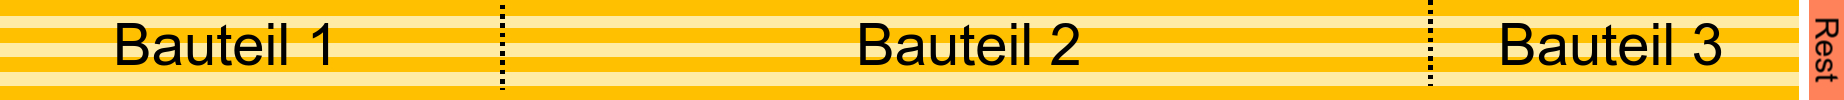
\includegraphics[width=1.00\textwidth, center]{Images/BalkenBauteileRest}\\
    \caption{Balken aus drei Bauteilen mit Rest, Sägelinien schwarz gepunktet}
    \label{figure:balkenbauteilerest}
\end{figure}

Balken werden vertikal in Pressen gestapelt und anschließend gepresst.
Eine mit Balken befüllte Presse, bei der festgelegt ist wie die Balken zu Bauteilen nach der Pressung zersägt werden müssen, nennt man auch Pressenplan.
In einem Pressenplan ist jedem Bauteil höchstens eine Position in einer Schicht (von unten gezählter Balken) einer Presse zugeordnet.
Folgend die Visualisierung eines Pressenplans für eine Presse:

\begin{figure}[h]
    \centering
    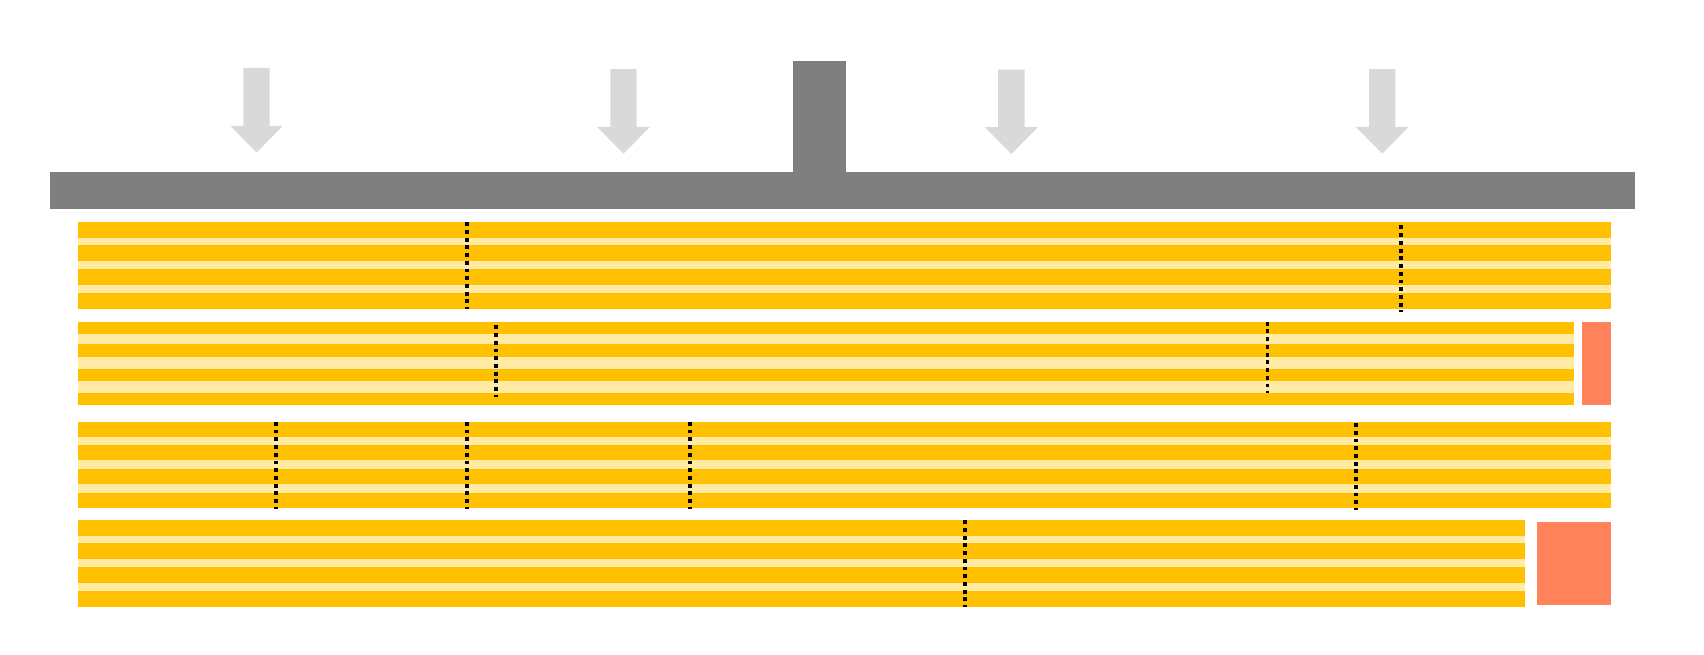
\includegraphics[width=1.00\textwidth, center]{Images/Pressenplan}\\
    \caption{Pressenplan für eine Presse mit vier Balken, 13 Bauteilen und zwei Reststücken \sem{Gern hier schon in der Skizze die Begriffe der Schicht und Position einführen, sowie Länge und Höhe definieren}}
    \label{figure:pressenplanproblem}
\end{figure}

Da Pressen im Allgemeinfall in einer Pressung nur Bauteile gleicher Breite pressen können, werden die Bauteile nach Breite vorsortiert.
Damit reduziert man die Dimension des Problems vom 3-Dimensionalen auf das 2-Dimensionale, da nur noch Länge und Höhe aller Entitäten berücksichtigt werden muss.

Die Eingabe für das Pressenplanungsproblem ist eine Liste von Bauteilen mit Länge und Höhe sowie deren Anzahl.
Diese Eingabe wird auch Auftrag genannt.
Die Lösung des Pressenplanungsproblems (Ausgabe) ist ein Pressenplan.
An einen Pressenplan bestehen folgende Anforderungen:
\begin{itemize}
    \item Pressen haben eine Minimal- und Maximalhöhe. Die Summe der Höhe aller Balken einer Presse muss in diesem Intervall liegen.
    \item Pressen haben eine Minimal- und Maximallänge. Die Länge aller Balken einer Presse muss in diesem Intervall liegen.
    \item Alle Balken einer Presse haben die gleiche Länge. Dazu kann der Balken so aus Bauteilen zusammengesetzt sein, dass ein Rest übrig bleibt.
    \item Alle Bauteile, die einen Balken formen, haben die gleiche Höhe.
    \item Jedes Bauteil eines Auftrages ist höchstens einem Balken zugeordnet.
    \item Jeder Balken ist genau einer Presse zugeordnet.
\end{itemize}

\sem{Ziele: Reste vermeiden, Pressen auslasten, Viel verplanen. Die Priorität der Zeile beeinflusst maßgeblich die Lösung. Was ist wichtiger Rest oder Anzahl Teile verplant?}

\sem{Versuche mal das Problem Einzuordnung in Schnittprobleme, bzw. Binpacking.}
% Hier könnte noch ein Beispiel eingefügt werden


\section{Modellierung}
\label{section:modellierung}
Mathematische Modelle für Erfüllbarkeit des Problems.
Warum zwei Modelle?
Größe des Problems (Unbekannte, Formeln)?

\section{Optimierung}
Erweiterung der Modelle um Optimierungsziele.
OMT, Incremental refinement, \ldots